%%%%%%%%%%%%%%%%%%%%%%%%%%%%%%%%%%%%%%%%%%%%%%%%%%%%%%%%%% 
\chapter{実行実験}\label{chap:experiment}
%%%%%%%%%%%%%%%%%%%%%%%%%%%%%%%%%%%%%%%%%%%%%%%%%%%%%%%%%% 
本章では,前章にて説明した3つの符号化
\textbf{undirected},\textbf{directed},\textbf{acyclicity}
の性能を評価するために
行った実験について説明し,その結果と考察を示す.
実験は,第\ref{chap:background}章にて説明した,ハミルトン閉路問題,最短ハミルトン路・閉路問題,コスト制約付きハミルトン路問題の3つをそれぞれ対象とした3回行った.

%%%%%%%%%%%%%%%%%%%%%%%%%%%%%%%%%%%%%%%%%%%%%%%%%%%%%%%%%%
\section{ハミルトン閉路問題}
%%%%%%%%%%%%%%%%%%%%%%%%%%%%%%%%%%%%%%%%%%%%%%%%%%%%%%%%%%

%%%%%%%%%%%%%%%%%%%%%%%%%%%%%%%%%%%%%%%%%%%%%%%
\begin{figure}[tb]
\begin{center}
  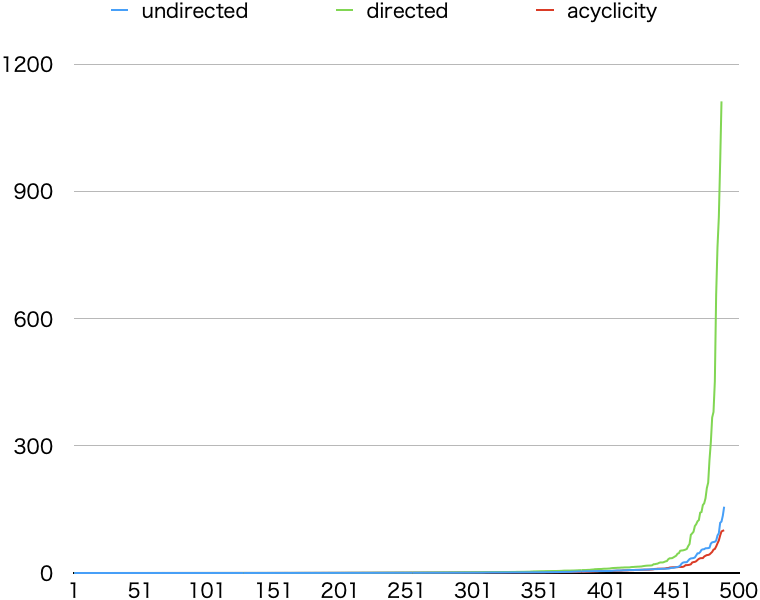
\includegraphics[width=10cm]{fig/cactus.png}
\caption{カクタスプロット1}
\label{cactus}
\end{center}
\end{figure}
%%%%%%%%%%%%%%%%%%%%%%%%%%%%%%%%%%%%%%%%%%%%%%%

%%%%%%%%%%%%%%%%%%%%%%%%%%%%%%%%%%%%%%%%%%%%%%%
\begin{table}[t]\scriptsize
  \centering
  %\tabcolsep = 0.8mm
  \renewcommand{\arraystretch}{1.2}
  \begin{tabular}{lr|rrr}
    問題サイズ & 問題数 & \textsf{undirected} & \textsf{directed} & \textsf{acyclicity}\\
   \hline
    $\:\:\:\:\:\,\, 0 \leq |V| < 1000$     & 171   & 156   & \alert{171}   & 156  \\ %
    $1000 \leq |V| < 2000$  & 165   & 120   & \alert{159}   & 121  \\
    $2000 \leq |V| < 3000$  & 177   & 125   & \alert{163}   & 80   \\
    $3000 \leq |V| < 4000$  & 185   & 104   & \alert{147}   & 48   \\
    $4000 \leq |V| < 5000$  & 128   & 92    & \alert{106}   & 30   \\
    $5000 \leq |V| < 6000$  & 80    & 63    & \alert{70}    & 21   \\
    $6000 \leq |V| < 7000$  & 55    & 39    & \alert{41}    & 20   \\
    $7000 \leq |V| < 8000$  & 28    & 12    & \alert{15}    & 4    \\
    $8000 \leq |V| < 9000$  & 10    & 2     & \alert{5}     & 1    \\
    $9000 \leq |V| < 10000$  & 2     & \alert{2}     & \alert{2}     & 1    \\
   \hline
    合計 & 1001 & 715   & \alert{879}   & 482  
  \end{tabular}
  \vskip .5em
%  \caption{ハミルトン閉路問題: 解けた問題数}
  \label{sat_table}
\end{table}
%label{sat_table}
%%%%%%%%%%%%%%%%%%%%%%%%%%%%%%%%%%%%%%%%%%%%%%%

%%%%%%%%%%%%%%%%%%%%%%%%%%%%%%%%%%%%%%%%%%%%%%%
\begin{figure}[tb]
\begin{center}
  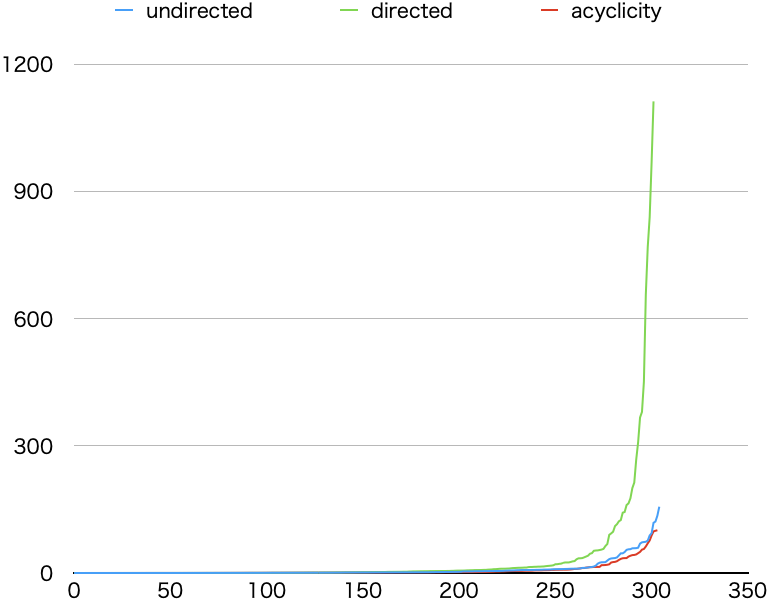
\includegraphics[width=10cm]{fig/cactussat.png}
\caption{SATのみのカクタスプロット}
\label{cactussat}
\end{center}
\end{figure}
%%%%%%%%%%%%%%%%%%%%%%%%%%%%%%%%%%%%%%%%%%%%%%%

%%%%%%%%%%%%%%%%%%%%%%%%%%%%%%%%%%%%%%%%%%%%%%%
\begin{figure}[tb]
\begin{center}
  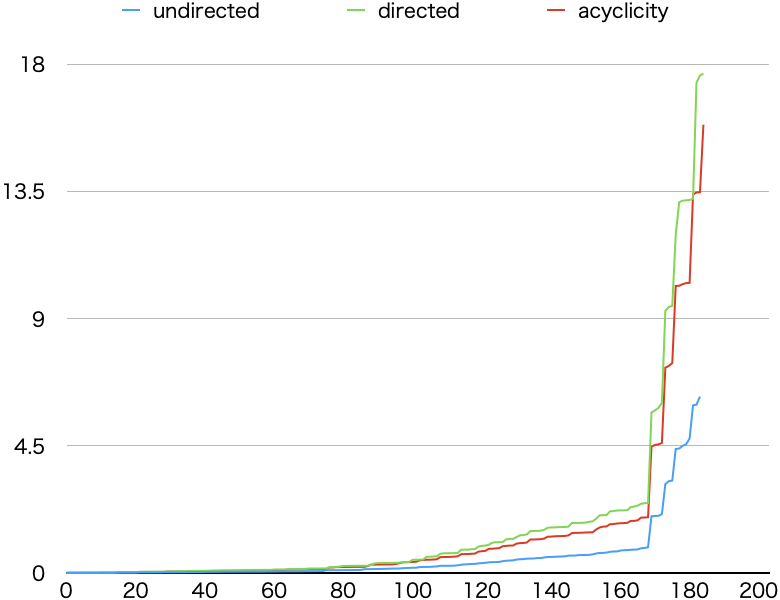
\includegraphics[width=10cm]{fig/cactusunsat.png}
\caption{UNSATのみのカクタスプロット}
\label{cactusunsat}
\end{center}
\end{figure}
%%%%%%%%%%%%%%%%%%%%%%%%%%%%%%%%%%%%%%%%%%%%%%%

まずはハミルトン閉路問題を対象とする実験について,
この実験では,様々な種類のグラフ上でのハミルトン閉路問題について
3つの符号化\textsf{undirected},\textsf{directed},\textsf{acyclicity}の性能を比較した.
以下では,実験の詳細,結果,考察について述べる.

\begin{itemize}
\item まずは,本実験で用いた6種類のベンチマーク問題について説明する.
それぞれ,color04,complete,knight,tsplib,grid,randomと呼ぶ.
\item grid以外は,
\textit{Incremental SAT-based Method with Native Boolean Cardinality Handling for the Hamiltonian Cycle Problem}\cite{soh14:jelia2014}の補足資料が載せられたwebページ\footnote{\url{https://tsoh.org/scarab/jelia2014/}}から手に入る.

\item color04は1993年秋に開催された\textit{DIMACS Computational Challenge}をベースとする
グラフ彩色問題の計算手法の研究を奨励する一連の活動
\textit{COLOR02/03/04}\footnote{\url{https://mat.tepper.cmu.edu/COLOR02/}}
が提供するグラフ彩色問題のインスタンスをそれぞれASPファクト形式に変換した127問,
\item completeは先述のwebページ\footnotemark[1]で提供されている完全グラフのインスタンスをASPファクト形式に変換した15問,
\item knightは騎士巡回問題(Knight's Tour)のインスタンスであり,
論文\cite{soh14:jelia2014}と同様に8x8,12x12,20x20,30x30,...100x100のマス目のものを用いた.
\item tsplibは,TSPLIBが提供するハミルトン閉路問題のインスタンス群\footnote{\url{http://comopt.ifi.uni-heidelberg.de/software/TSPLIB95/hcp/}}をASPファクト形式に変換したものであり,
\item gridは,自作した頂点数が6x6...10x10,12x12...17x17のグリッドグラフのインスタンスである.
\item randomは,先述のwebページ\footnotemark[1]にて提供されたランダムに生成されたグラフを表すインスタンスである.
\end{itemize}

解くのに使用したASPシステムは{\clingo}のver5.4.0であり,
オプションは\textit{trendy},一問あたりの時間制限を30分とした.
実験環境は,Mac mini Intel Corei7 3.2GHz 64GBメモリである.

まとめると,この実験では提案した3つのASP符号化\textsf{undirected},\textsf{directed},\textsf{acyclicity}を用いて
上記のベンチマーク問題をそれぞれ符号化し,一問あたりの制限時間を30分として,
{\clingo}で実行し,実行CPU時間などの結果を集計した.

\begin{itemize}
\item 3符号化の性能比較のため,集計した結果をカクタスプロットにしたものが図~\ref{cactus}である.
\item カクタスプロットは,縦軸が各問題を解くのかかったCPU時間,横軸は解けた問題数を表す.
\item カクタスプロット上では,グラフが右によるほど制限時間内に多くの問題を解けたことを示し,
  下によるほどより早く問題を解けたことを示すが,
  横軸で同じ値を示しても同じ問題を解いていることを示しているわけではないため注意が必要である.
\item 図~\ref{cactus}からわかるように,\textsf{acyclicity}がもっとも優秀な性能を示した.
\item ただし,\textsf{undirected}と\textsf{acyclicity}の間に大きな差が見られなかったため,
  表~\ref{sat_table}によって詳細を比較した.
\end{itemize}

\begin{itemize}
\item 表\ref{sat_table}は,ベンチマーク問題の種類ごとに解がSAT,UNSAT,UNKNとなった問題の数を表にしたものである.
\item \textsf{undirected}と\textsf{acyclicity}が制限時間内に解けなかった問題数はともに4問であったが,その内訳は\textsf{undirected}がcolor04の1問とgridの3問,\textsf{acyclicity}がcolor04の2問とgridの2問となった.
\item color04にて,\textsf{undirected}に解けて\textsf{acyclicity}に解けなかった問題では,変数の個数や一貫性制約の数において,その結果に反して\textsf{acyclicity}が少ない値を示したに.
\item しかし,{\clingo}が解く過程で\textsf{acyclicity}では,制限時間内のみで,\textsf{undirected}の約40倍もの選択が行われ,発生したコンフリクト数は約60倍であった.
\item 一方で,gridにて\textsf{acyclicity}に解けて\textsf{undirected}に解けなかった問題では,一貫性制約の数に大きな差はなかったが,変数の数において後者は前者の2倍であった.
\item さらに,{\clingo}が解く過程で発生した選択数は後者は前者の90倍以上であった.
\item 結果に差が生じた2問について,color04のものは解がSATであったが,gridの問題の解はUNSATであったため,図~\ref{cactus}を解がSATであったものと,UNSATのものに分けたものとに分けて集計したところ,それぞれ,図~\ref{cactussat}と図~\ref{cactusunsat}となった.
\item 図~\ref{cactussat}は図~\ref{cactus}と比べても,傾向に大差はなかったが,図~\ref{cactusunsat}では,\textsf{undirected}が優秀な成績を示している.
\item つまり,解がSATであるような問題では\textsf{acyclicity}が優秀であり,解がUNSATであるような問題では\textsf{undirected}が優秀であった.
\end{itemize}


%%%%%%%%%%%%%%%%%%%%%%%%%%%%%%%%%%%%%%%%%%%%%%%%%%%%%%%%%%
\section{最短ハミルトン路・閉路問題}
%%%%%%%%%%%%%%%%%%%%%%%%%%%%%%%%%%%%%%%%%%%%%%%%%%%%%%%%%%

%%%%%%%%%%%%%%%%%%%%%%%%%%%%%%%%%%%%%%%%%%%%%%%
\begin{table}[htbp]
  \caption{実験結果2-1:trendy}
  \label{min_table_tr}
  \centering
  \begin{tabular}{|l|rrr|}
    \hline
    Instance&undirected&directed&acyclicity \\
    \hline
    grid5&50,656*&50,656*&50,656* \\
    grid6&68,656*&68,656*&68,656* \\
    grid7&91,822*&91,822*&91,822* \\
grid8&113,250&\textcolor{red}{112,916}&113,277 \\
grid9&\textcolor{red}{142,502}&143,326&143,660 \\
grid10rc&\textcolor{red}{172,703}&174,866&175,999 \\
grid11&\textcolor{red}{200,399}&204,456&200,638 \\
grid12&\textcolor{red}{231,278}&239,275&232,012 \\
grid13&\textcolor{red}{276,692}&276,926&276,899 \\
grid14&317,617&\textcolor{red}{317,144}&317,676 \\
grid15&\textcolor{red}{375,906}&376,809&376,210 \\
grid16&421,249&\textcolor{red}{419,737}&423,753 \\
US48&11,698*&11,698*&11,698* \\
    \hline
  \end{tabular}
\end{table}
%\label{min_table_tr}
%%%%%%%%%%%%%%%%%%%%%%%%%%%%%%%%%%%%%%%%%%%%%%%

続いて,最短ハミルトン路・閉路問題について,3つの符号化の性能を比較した.

\begin{itemize}
\item ベンチマーク問題としては,12個のグリッドグラフと図~\ref{fig:USmap}の米国本土48州の隣接グラフを用いた.
\item 12個のグリッドグラフは,前章で用いたgridの11問に,頂点11x11のグリッドグラフを追加したものである.
\item グリッドグラフの各辺のコストは1000〜2000の範囲の一様ランダム整数値である.
\end{itemize}

解くのに使用したASPシステムは{\clingo}のver5.4.0であり,
オプションは\textit{trendy},一問あたりの時間制限を3時間とした.
実験環境は,Mac mini Intel Corei7 3.2GHz 64GBメモリである.

つまり,この実験では提案した3つのASP符号化\textsf{undirected},\textsf{directed},\textsf{acyclicity}を用いて
上記のベンチマーク問題をそれぞれ符号化し,一問あたりの制限時間を3時間として,
{\clingo}で実行した.結果として得られた時間内に求められたハミルトン路・閉路の最短距離を表~\ref{min_table_tr}にまとめた.

\begin{itemize}
\item 表~\ref{min_table_tr}では,問題ごとに各符号化が時間内に求められた最短距離を記した.
\item 赤文字が,3符号化を比較した際の最良値であり,*マークがその問題の最短距離が求められたことを表している.
\item したがって,grid5〜7とUS48では全ての符号化にて最短距離が時間内に求められた.
\item 表~\ref{min_table_tr}より,赤文字がもっとも多かった\textsf{undirected}が優秀な性能を示した.
\end{itemize}

%%%%%%%%%%%%%%%%%%%%%%%%%%%%%%%%%%%%%%%%%%%%%%%%%%%%%%%%%%
\section{コスト制約付きハミルトン路問題}
%%%%%%%%%%%%%%%%%%%%%%%%%%%%%%%%%%%%%%%%%%%%%%%%%%%%%%%%%%

%%%%%%%%%%%%%%%%%%%%%%%%%%%%%%%%%%%%%%%%%%%%%%%
\begin{table*}[tb]\footnotesize
  \tabcolsep = 2mm
  %\renewcommand{\arraystretch}{1.0}
  \vskip .5em
  \centering
  \begin{tabular}{lr|rrr}
    \hline
    閾値(倍率)    &	解の総数 & \textsf{undirected} & \textsf{directed} & \textsf{acyclicity} \\
    \hline
    11698(1.00)   &	1      &\textbf{2.979} & 7.531 & 4.586	\\
    11814(1.01)   &	8      &5.587  & 15.322	& \textbf{5.250}	\\
    11931(1.02)   &	28     &\textbf{3.243}& 18.600	& 3.578	\\
    12282(1.05)   &	388    &10.003&19.818	& \textbf{6.296}	\\
    12867(1.10)   &	16,180  &16.548& 28.555	& \textbf{9.764}\\
    14037(1.20)   &	939,209 &48.262       &40.717	& \textbf{26.837}\\
    15207(1.30)   &	4,525,541&88.172      &55.276	& \textbf{42.037}\\
    16377(1.40)   &	6,702,964&99.154       &47.647	& \textbf{40.640}	\\
    17547(1.50)   &	6,876,526&95.390       &45.265	& \textbf{38.411}	\\
    18716(1.60)   &	6,876,928&98.937       &49.138	& \textbf{40.748}	\\
    \hline
    平均CPU時間 &   & 46.8275 & 32.7869  & \textbf{21.8147}\\\hline
%    Best    &   & 2 & 0 & \textbf{8} \\ \hline
  \end{tabular}
  \vskip .5em
  \caption{コスト制約付きハミルトン路問題: 解の全列挙に要した CPU 時間}
  \label{cost_table}
\end{table*}
%\label{cost_table}
%%%%%%%%%%%%%%%%%%%%%%%%%%%%%%%%%%%%%%%%%%%%%%%

最後に,コスト制約付きハミルトン路問題について,3符号化を比較した.

\begin{itemize}
\item ベンチマーク問題として図~\ref{fig:USmap}の米国本土48州の隣接グラフを用いた.
\item 閾値は表\ref{cost_table}にあるように11698〜18716までの10の値を与えた.
\item 始点はWA,終点はMEとした.
\end{itemize}

解くのに使用したASPシステムは{\clingo}のver5.4.0であり,
オプションは\textit{crafty},一問あたりの時間制限を3時間とした.
実験環境は,Mac mini Intel Corei7 3.2GHz 64GBメモリである.

したがって,この実験では提案した3つのASP符号化\textsf{undirected},
\textsf{directed},\textsf{acyclicity}を用いて
上記のベンチマーク問題10問をそれぞれ符号化し,
一問あたりの制限時間を3時間として,{\clingo}で実行した.
結果として,問題ごとにかかったCPU時間を表~\ref{cost_table}にまとめた.

\begin{itemize}
\item 表~\ref{cost_table}では,各閾値におけるコスト制約を満たした
  ハミルトン路の数がModelsの列に記されており,
  その右に各符号化が解くのにかかったCPU時間が記されている.
\item 赤文字が3符号化の中での最短時間を表しており,タイムアウトは発生しなかった.
\item 10の閾値の内の7つにて\textsf{acyclicity}が最短時間で解いている.
\item 各閾値でかかったCPU時間の平均でも,\textsf{acyclicity}が最小である.
\item \textsf{acyclicity}がもっとも優秀であった.
\end{itemize}
%%%%%%%%%%%%%%%%%%%%%%%%%%%%%%%%%%%%%%%%%%%%%%%%%%%%%%%%%%

%%% Local Variables:
%%% mode: latex
%%% TeX-master: "paper"
%%% End:
